\documentclass[aspectratio=43]{beamer}
% \documentclass[aspectratio=169]{beamer}

% Title --------------------------------------------
\title[]{\huge Quantitative Research Workflow}
\author[]{Francisco Villamil}
\date[]{UC3M -- \today}

%%% NOTE -- CHECK THIS: https://github.com/paulgp/beamer-tips


%%% Building heavily on https://github.com/kylebutts/templates

% xcolor, define them
\usepackage{xcolor}

% TEXT COLORS
\definecolor{red}{HTML}{9a2515}
\definecolor{yellow}{HTML}{EBC944}
\definecolor{asher}{HTML}{555F61}
\definecolor{jet}{HTML}{131516}

% THEME COLORS
\definecolor{accent}{HTML}{107895}
\definecolor{accent2}{HTML}{9a2515}

% Color commands
\newcommand\red[1]{{\color{red}#1}}
\newcommand\yellow[1]{{\color{yellow}#1}}
\newcommand\asher[1]{{\color{asher}#1}}

\newcommand\BGred[1]{{\colorbox{red!80!white}{#1}}}
\newcommand\BGyellow[1]{{\colorbox{yellow!80!white}{#1}}}
\newcommand\BGasher[1]{{\colorbox{asher!80!white}{#1}}}

% to use only in some slides
\renewcommand<>{\BGyellow}[1]{\only#2{\beameroriginal{\BGyellow}}{#1}}

% Appendix numbering
\usepackage{appendixnumberbeamer}
% Math equations
\usepackage{amsmath}

% Beamer Options -------------------------------------

% Background
\setbeamercolor{background canvas}{bg = white}

% Change text margins
\setbeamersize{text margin left = 25pt, text margin right = 15pt}

% \alert
\setbeamercolor{alerted text}{fg = accent2}

% Frame title
\setbeamercolor{frametitle}{bg = white, fg = jet}
\setbeamercolor{framesubtitle}{bg = white, fg = accent}
\setbeamerfont{framesubtitle}{size = \small, shape = \itshape}

% Block
\setbeamercolor{block title}{fg = white, bg = accent2}
\setbeamercolor{block body}{fg = jet, bg = jet!10!white}

% Title page
\setbeamercolor{title}{fg = jet}
\setbeamercolor{subtitle}{fg = accent}

%% Custom \maketitle and \titlepage
\setbeamertemplate{title page}
{
    \begin{centering}
      % \vspace{20mm}
      {\Large \usebeamerfont{title}\usebeamercolor[fg]{title}\inserttitle}\\ \vskip0.25em%
      \ifx\insertsubtitle\@empty%
      \else%
        {\usebeamerfont{subtitle}\usebeamercolor[fg]{subtitle}\insertsubtitle\par}%
      \fi%
      {\vspace{10mm}\insertauthor}\\
      \ifx\insertinstitute\@empty%
      \else%
        {\vspace{5mm}\color{asher}\scriptsize{\insertinstitute}}\\\vspace{5mm}
      \fi%
      {\color{asher}\small{\insertdate}}\\
    \end{centering}
}

% Table of Contents
\setbeamercolor{section in toc}{fg = accent!70!jet}
\setbeamercolor{subsection in toc}{fg = jet}

% Button
\setbeamercolor{button}{bg = accent}

% Remove navigation symbols
\setbeamertemplate{navigation symbols}{}

% Table and Figure captions
\setbeamercolor{caption}{fg=jet!70!white}
\setbeamercolor{caption name}{fg=jet}
\setbeamerfont{caption name}{shape = \itshape}

% Put slide number / total slides at the bottom right
\makeatother
\makeatletter
\setbeamertemplate{footline} %{\hfill\insertframenumber/\inserttotalframenumber}
{%
  \leavevmode%
  \hbox{
  \begin{beamercolorbox}[wd=\paperwidth,ht=2.5ex,dp=1.125ex,leftskip=.3cm,rightskip=.3cm plus1fil]{footlinecolor}%
    \color{asher}{{\let\hyperlink\@secondoftwo\insertshorttitle}\hfill\insertshortauthor\hfill\insertshortdate\hfill\insertframenumber/\inserttotalframenumber}
  \end{beamercolorbox}}%
  \vskip0pt%
}
\makeatother
\makeatletter

% Bullet points

%% Fix left-margins
\settowidth{\leftmargini}{\usebeamertemplate{itemize item}}
\addtolength{\leftmargini}{\labelsep}

%% enumerate item color
\setbeamercolor{enumerate item}{fg = accent}
\setbeamerfont{enumerate item}{size = \small}
\setbeamertemplate{enumerate item}{\insertenumlabel.}

%% itemize
\setbeamercolor{itemize item}{fg = accent!70!white}
\setbeamerfont{itemize item}{size = \small}
\setbeamertemplate{itemize item}[circle]
\setlength{\itemsep}{0pt plus 6pt}

%% right arrow for subitems
\setbeamercolor{itemize subitem}{fg = accent!60!white}
\setbeamerfont{itemize subitem}{size = \small}
\setbeamertemplate{itemize subitem}{$\rightarrow$}

\setbeamertemplate{itemize subsubitem}[square]
\setbeamercolor{itemize subsubitem}{fg = jet}
\setbeamerfont{itemize subsubitem}{size = \small}

% References

%% Bibliography Font, roughly matching aea
\setbeamerfont{bibliography item}{size = \footnotesize}
\setbeamerfont{bibliography entry author}{size = \footnotesize, series = \bfseries}
\setbeamerfont{bibliography entry title}{size = \footnotesize}
\setbeamerfont{bibliography entry location}{size = \footnotesize, shape = \itshape}
\setbeamerfont{bibliography entry note}{size = \footnotesize}

\setbeamercolor{bibliography item}{fg = jet}
\setbeamercolor{bibliography entry author}{fg = accent!60!jet}
\setbeamercolor{bibliography entry title}{fg = jet}
\setbeamercolor{bibliography entry location}{fg = jet}
\setbeamercolor{bibliography entry note}{fg = jet}

%% Remove bibliography symbol in slides
\setbeamertemplate{bibliography item}{}





% Links ----------------------------------------------

\usepackage{hyperref}
\hypersetup{
  colorlinks = true,
  linkcolor = accent2,
  filecolor = accent2,
  urlcolor = accent2,
  citecolor = accent2,
}


% Line spacing --------------------------------------
\usepackage{setspace}
\setstretch{1.2}


% \begin{columns} -----------------------------------
\usepackage{multicol}


% % Fonts ---------------------------------------------
% % Beamer Option to use custom fonts
% \usefonttheme{professionalfonts}
%
% % \usepackage[utopia, smallerops, varg]{newtxmath}
% % \usepackage{utopia}
% \usepackage[sfdefault,light]{roboto}
%
% % Small adjustments to text kerning
% \usepackage{microtype}



% Remove annoying over-full box warnings -----------
\vfuzz2pt
\hfuzz2pt


% Table of Contents with Sections
\setbeamerfont{myTOC}{series=\bfseries, size=\Large}
\AtBeginSection[]{
        \frame{
            \frametitle{Roadmap}
            \tableofcontents[current]
        }
    }


% References ----------------------------------------
\usepackage[
    citestyle= authoryear,
    style = authoryear,
    natbib = true,
    backend = biber
]{biblatex}

% Smaller font-size for references
\renewcommand*{\bibfont}{\small}

% Remove "In:"
\renewbibmacro{in:}{}

% Color citations for slides
\newenvironment{citecolor}
    {\footnotesize\begin{color}{accent2}}
    {\end{color}}

\newcommand{\citetcolor}[1]{{\footnotesize\textcolor{asher}{\citet{#1}}}}
\newcommand{\citepcolor}[1]{{\footnotesize\textcolor{asher}{\citep{#1}}}}

% Tables -------------------------------------------
% Tables too big
% \begin{adjustbox}{width = 1.2\textwidth, center}
\usepackage{adjustbox}
\usepackage{array}
\usepackage{threeparttable, booktabs, adjustbox}

% Fix \input with tables
% \input fails when \\ is at end of external .tex file

\makeatletter
\let\input\@@input
\makeatother

% Tables too narrow
% \begin{tabularx}{\linewidth}{cols}
% col-types: X - center, L - left, R -right
% Relative scale: >{\hsize=.8\hsize}X/L/R
\usepackage{tabularx}
\newcolumntype{L}{>{\raggedright\arraybackslash}X}
\newcolumntype{R}{>{\raggedleft\arraybackslash}X}
\newcolumntype{C}{>{\centering\arraybackslash}X}

% Figures

% \imageframe{img_name} -----------------------------
% from https://github.com/mattjetwell/cousteau
\newcommand{\imageframe}[1]{%
    \begin{frame}[plain]
        \begin{tikzpicture}[remember picture, overlay]
            \node[at = (current page.center), xshift = 0cm] (cover) {%
                \includegraphics[keepaspectratio, width=\paperwidth, height=\paperheight]{#1}
            };
        \end{tikzpicture}
    \end{frame}%
}

% subfigures
\usepackage{subfigure}


% Highlight slide -----------------------------------
% \begin{transitionframe} Text \end{transitionframe}
% from paulgp's beamer tips
\newenvironment{transitionframe}{
    \setbeamercolor{background canvas}{bg=accent!60!black}
    \begin{frame}\color{accent!10!white}\LARGE\centering
}{
    \end{frame}
}


% Table Highlighting --------------------------------
% Create top-left and bottom-right markets in tabular cells with a unique matching id and these commands will outline those cells
\usepackage[beamer,customcolors]{hf-tikz}
\usetikzlibrary{calc}
\usetikzlibrary{fit,shapes.misc}

% To set the hypothesis highlighting boxes red.
\newcommand\marktopleft[1]{%
    \tikz[overlay,remember picture]
        \node (marker-#1-a) at (0,1.5ex) {};%
}
\newcommand\markbottomright[1]{%
    \tikz[overlay,remember picture]
        \node (marker-#1-b) at (0,0) {};%
    \tikz[accent!80!jet, ultra thick, overlay, remember picture, inner sep=4pt]
        \node[draw, rectangle, fit=(marker-#1-a.center) (marker-#1-b.center)] {};%
}


\begin{document}
% ====================================================

% ----------------------------------------------------
\begin{frame}
  \titlepage
\end{frame}
% ----------------------------------------------------

% ----------------------------------------------------
\begin{frame}
\frametitle{Thinking about workflow}
\centering

\begin{itemize}
  \item How you organize your coding projects: data, output, integration between different things (e.g. R and Latex)
  \begin{itemize}
    \item (Note on R Markdown)
  \end{itemize}
  \item How to code better
  \item Learning how to use a computer properly
 \end{itemize}

\end{frame}
% ----------------------------------------------------
  

% ----------------------------------------------------
\begin{frame}
\frametitle{Why?}
\centering

\begin{itemize}
  \item[1.] \textbf{Automate stuff:} you spend a lot of time on the computer so make it work for you
  \item[2.] \textbf{Avoid errors:} we should not trust ourselves
\end{itemize}

\end{frame}
% ----------------------------------------------------

% ----------------------------------------------------
\begin{frame}
\frametitle{Problems}
\centering

\begin{itemize}
\setbeamercovered{transparent}
  \item<1-> Version control: \texttt{final.docx}, \texttt{final2.docx}, \texttt{finalFINAL.docx}
  \item<2-> Going back to old (or not so old) projects and...
  \begin{itemize}
    \item change something in one 5000-line R file
    \item doesn't run because file is missing, where's the file?
    \item need to change some \textit{constant} and spend a whole day looking for it
  \end{itemize}
  \item<3-> Re-running versions of graphs and tables in the final dissertation
  \item<4-> Avoiding this things: \href{https://journals.sagepub.com/doi/10.1177/20531680221126454}{journals.sagepub.com/doi/10.1177/20531680221126454}
\end{itemize}

\end{frame}
% ----------------------------------------------------

% ----------------------------------------------------
\begin{frame}
\frametitle{Main ideas}
\centering

\begin{itemize}
  \item[1.] Working with \textbf{plain text} files
  \item[2.] Organizing coding and empirical projects
  \item[3.] Coding better (automating, defining constants, checks \& warnings...)
  \item[4.] Use version control (git)
  \item[5.] Use your tools better: learn some command line, customize computer, choose a text editor...
\end{itemize}

\end{frame}
% ----------------------------------------------------
  
% ----------------------------------------------------
\begin{frame}
\frametitle{Some resources}
\centering

\begin{itemize}
  \item Hadley Wickham's \href{http://adv-r.had.co.nz/Style.html}{R Style guide} (and the whole \href{http://adv-r.had.co.nz/}{Advanced R book} later on)
    \item Kieran Healy's \textit{The Plain Person’s Guide to Plain Text Social Science}: \href{https://plain-text.co/}{https://plain-text.co/}
  \begin{itemize}
    \item Although \texttt{emacs} is perhaps a bit too hardcore
  \end{itemize}
  \item The best Git course I know is this: \href{https://gitexercises.fracz.com/}{https://gitexercises.fracz.com/}
  \item MIT's \textit{The Missing Semester of Your CS Education}: \href{https://missing.csail.mit.edu/}{https://missing.csail.mit.edu/}
  \item Software Carpentry's lessons: \href{https://software-carpentry.org/lessons/}{https://software-carpentry.org/lessons/}
  \begin{itemize}
    \item Especially \href{https://swcarpentry.github.io/shell-novice/}{Unix Shell} and \href{https://swcarpentry.github.io/git-novice/}{Version Control with Git}
  \end{itemize}
  \item \href{https://github.com/franvillamil/workflow_example}{\textbf{github.com/franvillamil/workflow\_example}}
\end{itemize}

\end{frame}
% ----------------------------------------------------

% ----------------------------------------------------
\begin{frame}
\frametitle{What is \textbf{plain text}?}
\centering

% ----------------------------------------------------

\includegraphics[width = 0.5\textwidth]{img/xkcd}
% ----------------------------------------------------
  

\end{frame}
% ----------------------------------------------------
  

\section{Coding better and organizing data projects}

% ----------------------------------------------------
\begin{frame}
\frametitle{Coding projects: tasks as folders}
\centering

\begin{itemize}
  \item This applies especially to the R part of projects
  \item Do not create one huge R code file, use different files for different tasks
  \item You want to do the same with the folder structure
  \begin{itemize}
    \item \textbf{Especially with R output!}
  \end{itemize}
  \item (Optionally, you can use \textit{Makefile}, but it can be problematic)
\end{itemize}

\end{frame}
% ----------------------------------------------------

% ----------------------------------------------------
\begin{frame}
\frametitle{Coding projects: tasks as folders}
\centering

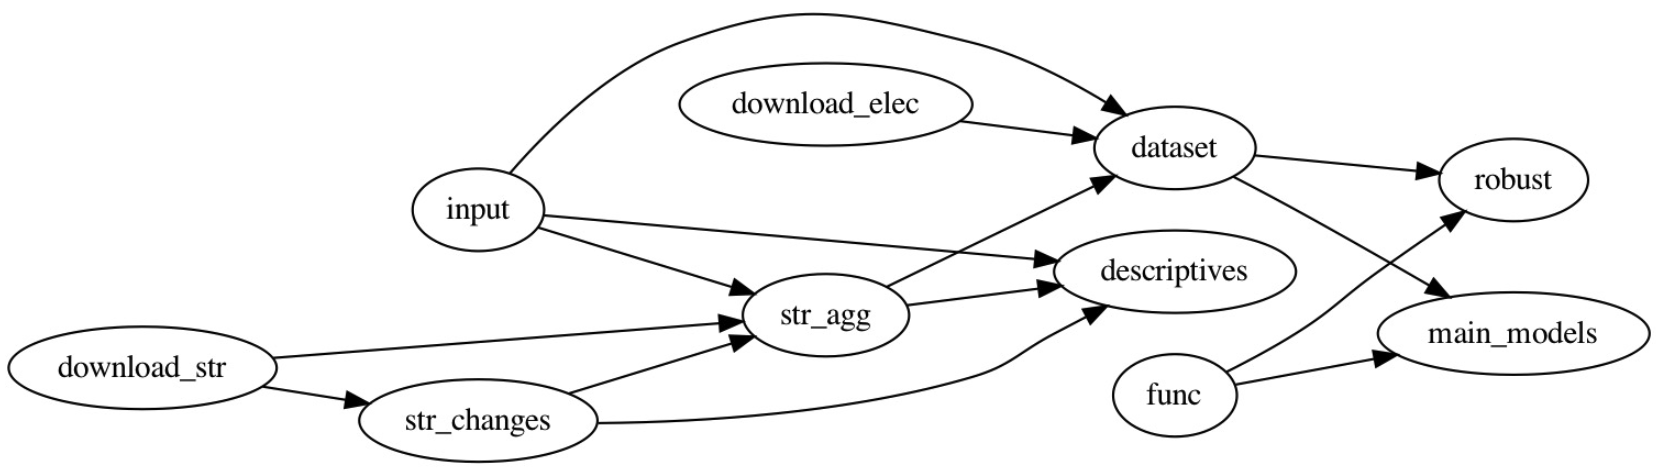
\includegraphics[width = \textwidth]{img/workflow_vox_streets}

\end{frame}
% ----------------------------------------------------

% ----------------------------------------------------
\begin{frame}
\frametitle{Coding projects extra: filenaming}
\centering

\begin{itemize}
  \item Not a lot of things here, but just think about how you name files or folders
  \item[1.] Do not use spaces
  \item[2.] Ideally use some standards (e.g. \texttt{1\_clean-file.R}, \texttt{2\_merge.R} ...)
  \item \textbf{{\color{red}{DON'T:}}} \texttt{First file.csv}, \textbf{definitely not:} \texttt{Datos educación.csv}
  \begin{itemize}
    \item good: \texttt{first\_file.csv}, \texttt{datos\_educacion.csv} etc
  \end{itemize}
\end{itemize}

\end{frame}
% ----------------------------------------------------

% ----------------------------------------------------
\begin{frame}
\frametitle{Coding projects, extra: integrate}
\centering

\begin{itemize}
  \item Put together \texttt{Latex} and \texttt{R} parts (and/or Python, etc)
  \item If you organize the folder as I said before, it's pretty much solved
  \item Overleaf example
  \item What you get with this? Avoid mistakes, makes your life easier...
\end{itemize}

\end{frame}
% ----------------------------------------------------

% ----------------------------------------------------
\begin{frame}
\frametitle{Coding projects, extra: Makefile}
\centering

\begin{itemize}
  \item Example
  \item \href{https://makefiletutorial.com/}{https://makefiletutorial.com/}
\end{itemize}

\end{frame}
% ----------------------------------------------------

% ----------------------------------------------------
\begin{frame}
\frametitle{Writing code I: automate via functions}
\centering

\begin{itemize}
  \item Main idea: you should not write the same code \textit{twice}
  \item Use functions to automate everything: producing plots, analyses (e.g. predicted probabilities), recurrent actions, etc
  \item Why? Avoids mistakes, easier to debug, cleaner files
  \item Examples:
  \begin{itemize}
    \item \href{github.com/franvillamil/ethnicity_vox/tree/master/func}{https://github.com/franvillamil/ethnicity\_africa/tree/master/func}
    \item \href{github.com/franvillamil/streets_vox/tree/master/func}{https://github.com/franvillamil/streets\_vox/tree/master/func}
  \end{itemize}
\end{itemize}

\end{frame}
% ----------------------------------------------------

% ----------------------------------------------------
\begin{frame}
\frametitle{Writing code II: write checks and warnings}
\centering

\begin{itemize}
  \item As you write code, always write checks using \texttt{stop()} or \texttt{warning()}, e.g.:
  \begin{itemize}
    \item if a new data frame is built from merging, what should be the number of rows in the final df? or columns?
    \item should two objects be identical?
    \item do we have duplicated values by some ID?
    \item do you expect \texttt{``145``} or \texttt{145} (character vs integer)?
    \item ...
    \item[]
  \end{itemize}
\end{itemize}

\end{frame}
% ----------------------------------------------------

% ----------------------------------------------------
\imageframe{img/stop1}
% ----------------------------------------------------

% ----------------------------------------------------
\imageframe{img/stop2}
% ----------------------------------------------------

% ----------------------------------------------------
\begin{frame}
\frametitle{Writing code II: write checks and warnings}
\centering

\begin{itemize}
\item Also try to minimize errors, e.g. that you have visuals of real output, e.g.:
\item[1.] I use \texttt{print()} all the time to show length of stuff, number of missing data, etc
\item[2.] \texttt{modelsummary} vs \texttt{stargazer} example
  \begin{itemize}
    \item \href{https://journals.sagepub.com/doi/10.1177/20531680221126454}{journals.sagepub.com/doi/10.1177/20531680221126454}
    \item \href{https://github.com/franvillamil/streets_vox/blob/master/robust/rob.R}{github.com/franvillamil/streets\_vox/blob/master/robust/rob.R}
  \end{itemize}
\end{itemize}

\end{frame}
% ----------------------------------------------------

\section{Using computers}

% ----------------------------------------------------
\begin{frame}
\frametitle{Plain text}
\centering

\begin{itemize}
  \item Quicker and easier to work with
  \item Cross-platform and does not depend on proprietary software
  \item Much better for the things you want to do
  \begin{itemize}
    \item You can use version control on it
    \item Closer to how machines work it - so easier for whatever related to machines (e.g. syncing two computers) $\rightarrow$ \href{https://github.com/franvillamil/configfiles}{example1}, \href{https://github.com/franvillamil/sublime_settings}{example2}
    \item It's a base ingredient you can convert into whatever (e.g. with \texttt{R}, \texttt{LaTeX}, etc)
  \end{itemize}
\end{itemize}

\end{frame}
% ----------------------------------------------------

% ----------------------------------------------------
\begin{frame}
\frametitle{Customizing your computer}
\centering

\begin{itemize}
  \item \href{https://franvillamil.github.io/posts/setup_macos.html}{https://franvillamil.github.io/posts/setup\_macos.html}
  \item \href{https://github.com/franvillamil/templates}{https://github.com/franvillamil/templates}
  \item \href{https://github.com/franvillamil/configfiles}{https://github.com/franvillamil/configfiles}
  \item Examples: mdtopdf/docxtopdf, baserepos, Spectacle, ...
\end{itemize}

\end{frame}
% ----------------------------------------------------

% ----------------------------------------------------
\begin{frame}
\frametitle{Code editor}
\centering

\begin{itemize}
  \item Choose and get used to some code editor
  \begin{itemize}
    \item You're probably using the editor in \texttt{RStudio}, that's fine, but there are reasons to use better and more general tools
  \end{itemize}
  \item You can customize these so suit your needs, e.g.:
  \begin{itemize}
    \item Edit \& run languages you use (\texttt{R}, \texttt{Latex}, whatever)
    \item Small stuff that saves time, like snippets
    \item Navigate a project
    \item And much more complicated stuff we're not going to talk about and that I do not know so much about
  \end{itemize}
  \item I use Sublime Text: \href{https://www.sublimetext.com/}{https://www.sublimetext.com/}
  \item Anyway, \textbf{don't use MS Word} (as much as possible)
\end{itemize}

\end{frame}
% ----------------------------------------------------

% ----------------------------------------------------
\begin{frame}
\frametitle{Using the command line}
\centering

\begin{itemize}
  \item Think of it as the language to communicate with the OS
  \item No need that you become a computer wizard, but I personally think it pays off to learn a little bit
  \item Why?
  \begin{itemize}
    \item Automate stuff in the computer (e.g. from updating local files to converting .docx into pdf)
    \item Navigate and work with files faster
    \item Version control, installing stuff, solving issues
    \item Virtual machines
  \end{itemize}
  \item \textbf{Note:} Unix/Mac vs Windows
\end{itemize}

\end{frame}
% ----------------------------------------------------

% ----------------------------------------------------
\begin{frame}
\frametitle{Version control (Git)}
\centering

\begin{itemize}[<+->]
  \item \texttt{final1.docx}, \texttt{finalfinal.docx}... but in a proper way
  \item You want to keep control of all versions of a file, something like MS Word's `Tracked changes' but just much better
  \begin{itemize}
    \item Keep a time machine of all versions of a file
    \item Allow collaboration between different people (or between two computers)
  \end{itemize}
  \item There is more than one system, but most people use \texttt{Git} (and Github)
\end{itemize}

\end{frame}
% ----------------------------------------------------

% ----------------------------------------------------
\begin{frame}
\frametitle{Version control}
\centering

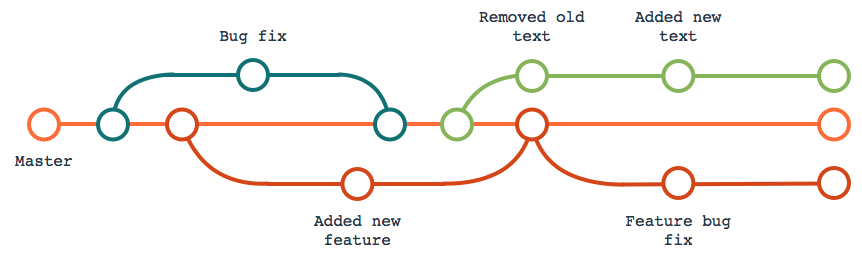
\includegraphics[width = \textwidth]{img/gitesquema}

\end{frame}
% ----------------------------------------------------

% ----------------------------------------------------
\begin{frame}
\frametitle{Version control}
\centering

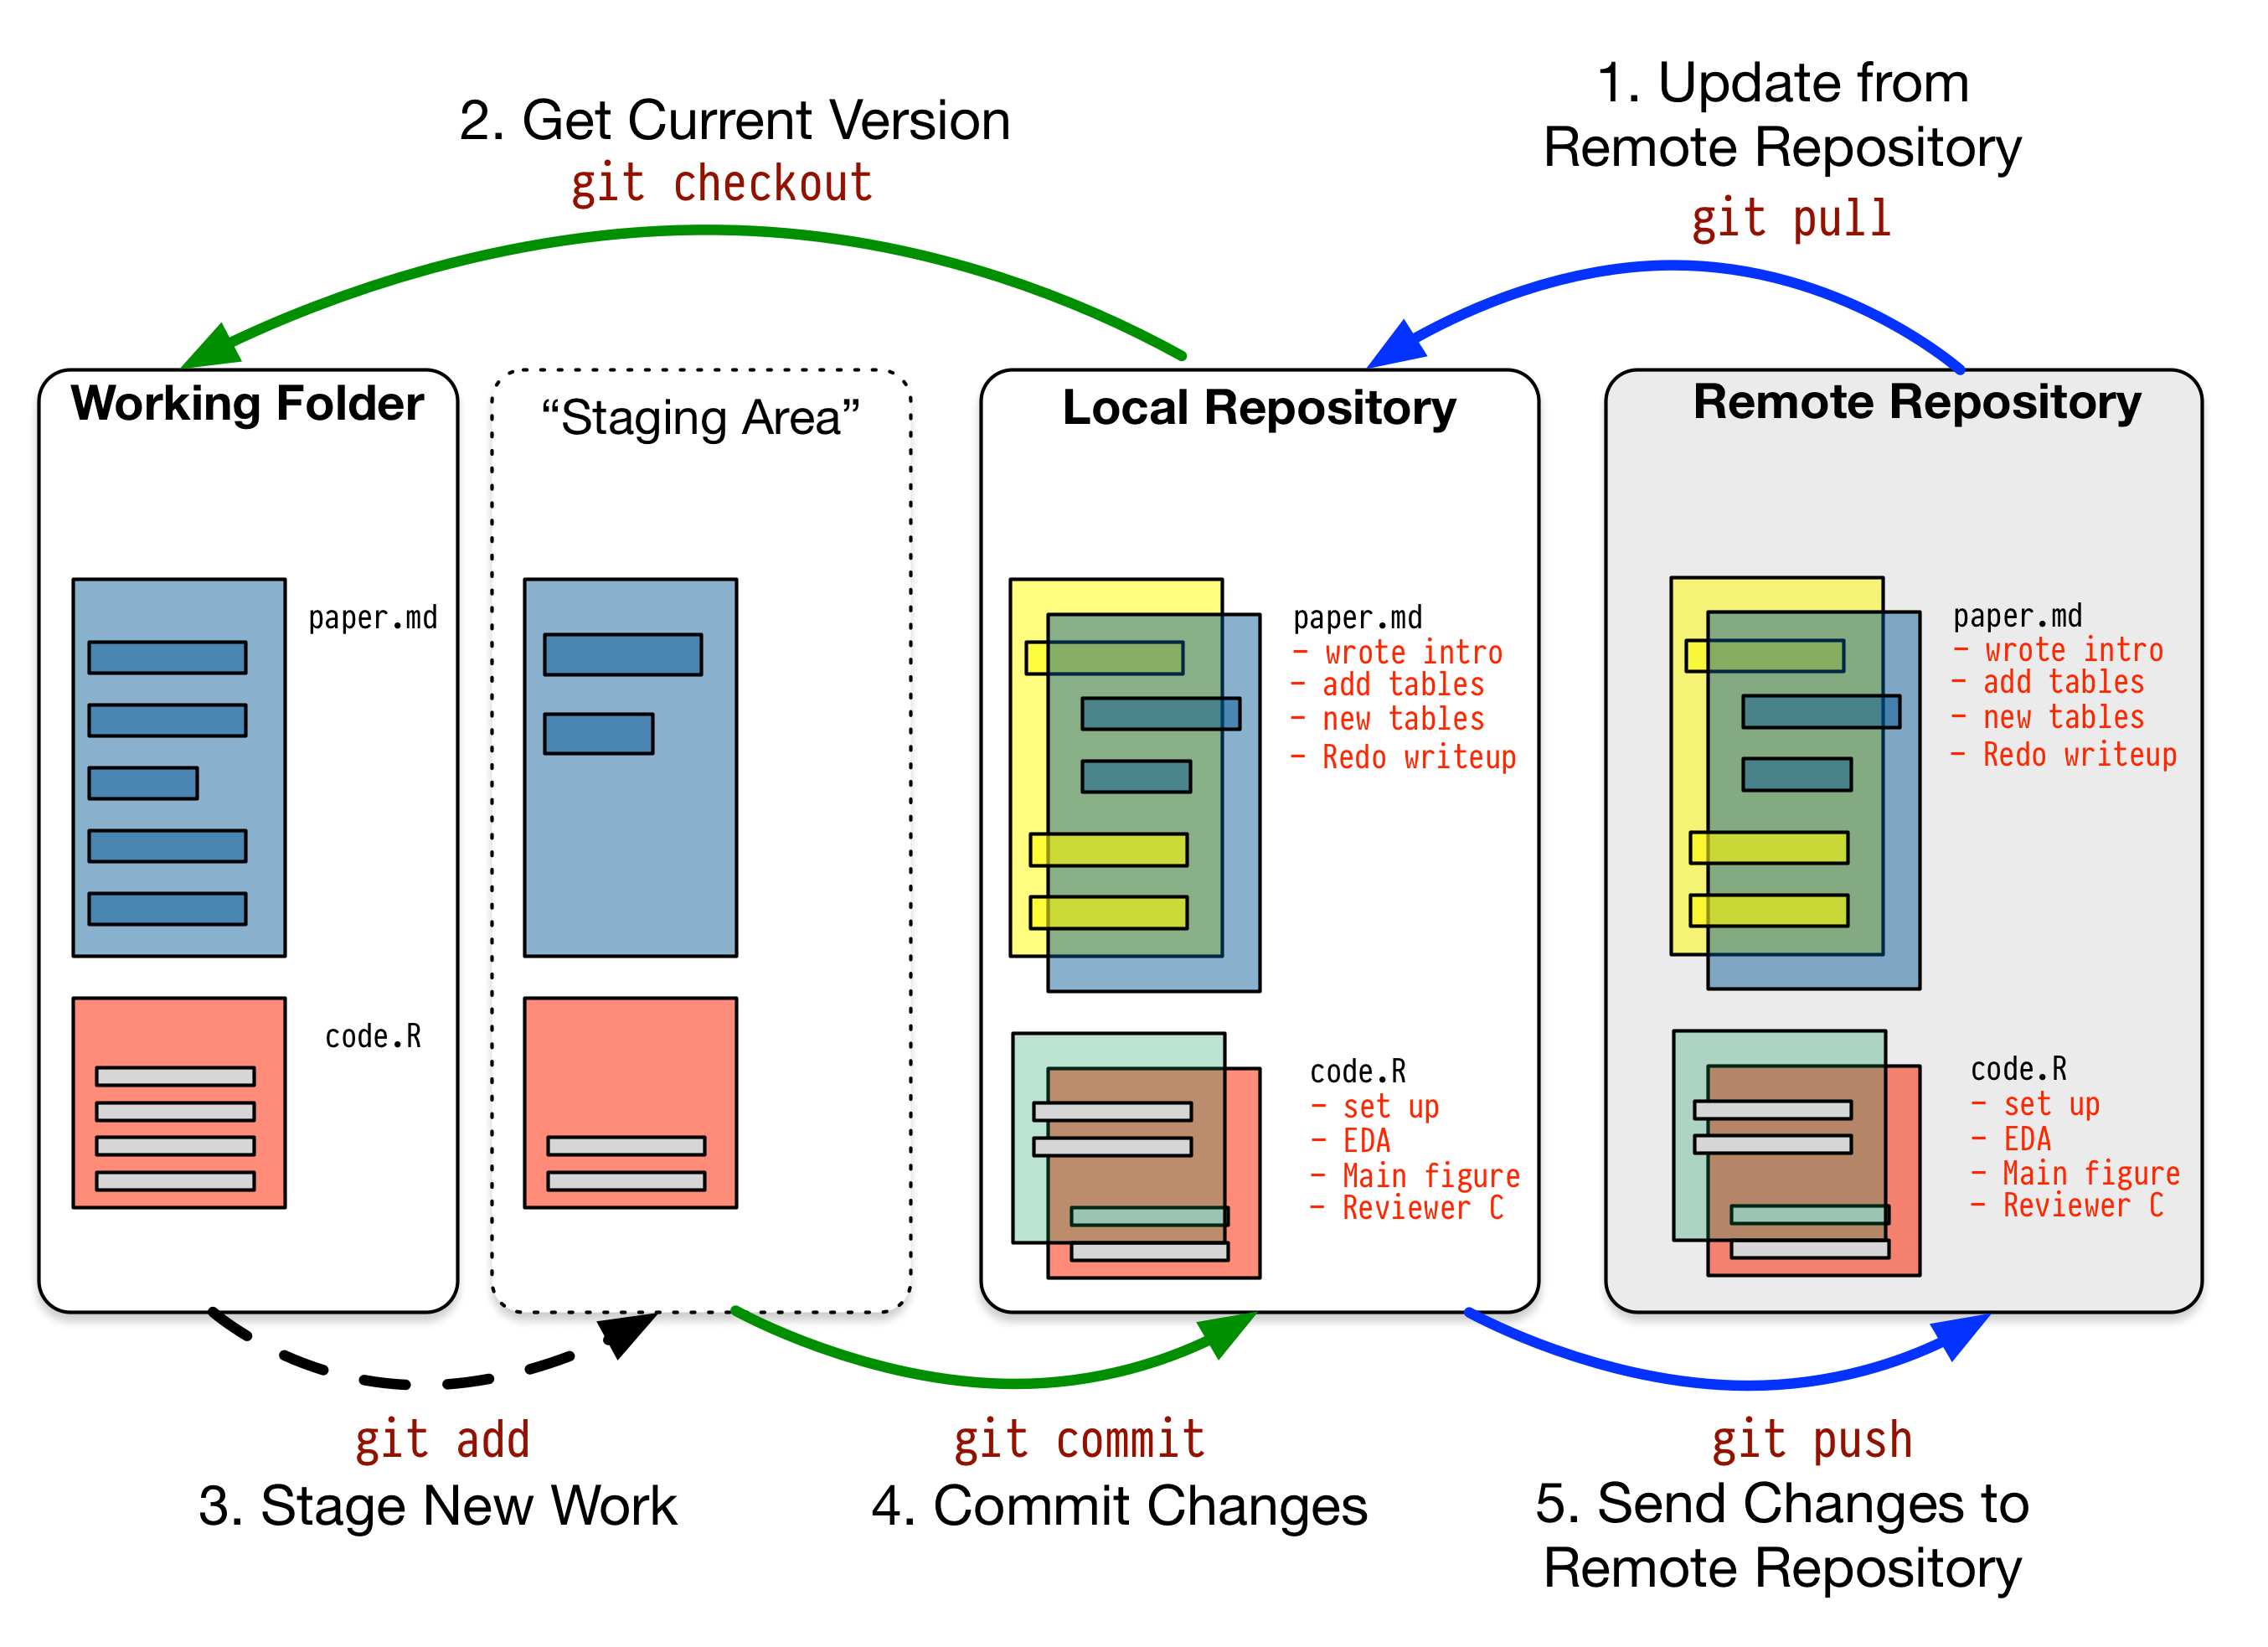
\includegraphics[width = \textwidth]{img/git-basic}

\end{frame}
% ----------------------------------------------------

% ----------------------------------------------------
\begin{frame}
\frametitle{Version control - a note}
\centering

\begin{itemize}
  \item Version control works \textbf{much} better if you work with other people who also use version control, which is often not the case (at least not mine)
  \item Yet, there are two advantages to use it in my view:
  \begin{itemize}
    \item Obvious one: keep older versions of a file
    \item If you work with two computers, perhaps Google Drive/Dropbox do not work that well
    \item Virtual machines (e.g. Google Cloud Computing, Amazon Web Services)
  \end{itemize}
\end{itemize}

\end{frame}
% ----------------------------------------------------

%\appendix
%\renewcommand{\theframenumber}{A\arabic{framenumber}}
%\renewcommand{\insertframenumber}{A\arabic{framenumber}}

% ====================================================
\end{document}
